\documentclass[conference]{IEEEtran}
\IEEEoverridecommandlockouts
% The preceding line is only needed to identify funding in the first footnote. If that is unneeded, please comment it out.
\usepackage{cite}
\usepackage{amsmath,amssymb,amsfonts}
\usepackage{algorithmic}
\usepackage{graphicx}
\usepackage{textcomp}
\usepackage{xcolor}
\def\BibTeX{{\rm B\kern-.05em{\sc i\kern-.025em b}\kern-.08em
    T\kern-.1667em\lower.7ex\hbox{E}\kern-.125emX}}
\begin{document}

\title{Effect of Injection Timing and Valve Timing on Combustion Characteristics and Performance of Port-Fueled Hydrogen Internal Combustion Engines\\
% {\footnotesize \textsuperscript{*}Note: Sub-titles are not captured in Xplore and
% should not be used}
}

\author{\IEEEauthorblockN{Isuru Wickramaarachchi}
\IEEEauthorblockA{\textit{Department of Mechanical Engineering} \\
\textit{University of Moratuwa}\\
Katubedda, Sri Lanka \\
waisurumangala@gmail.com}
\and
\IEEEauthorblockN{Isuru Wickramaarachchi}
\IEEEauthorblockA{\textit{Department of Mechanical Engineering} \\
\textit{University of Moratuwa}\\
Katubedda, Sri Lanka \\
waisurumangala@gmail.com}
\and
\IEEEauthorblockN{Isuru Wickramaarachchi}
\IEEEauthorblockA{\textit{Department of Mechanical Engineering} \\
\textit{University of Moratuwa}\\
Katubedda, Sri Lanka \\
waisurumangala@gmail.com}
\and
\IEEEauthorblockN{Isuru Wickramaarachchi}
\IEEEauthorblockA{\textit{Department of Mechanical Engineering} \\
\textit{University of Moratuwa}\\
Katubedda, Sri Lanka \\
waisurumangala@gmail.com}
\and
\IEEEauthorblockN{Isuru Wickramaarachchi}
\IEEEauthorblockA{\textit{Department of Mechanical Engineering} \\
\textit{University of Moratuwa}\\
Katubedda, Sri Lanka \\
waisurumangala@gmail.com}
}

\maketitle

\begin{abstract}
Combustion Characteristics are affeced by valve and injection timing in H\textsubscript{2} engines.
\end{abstract}

\begin{IEEEkeywords}
valve, injection, combustion characteristics, hydrogen, port-fuelled
\end{IEEEkeywords}

\section{Introduction}
Due to global warming, hydrogen is getting popular as an alternative fuel. It is suggested that abnormal combustion, which is a major problem in hydrogen engines, can be controlled by changing design parameters including valve timing, injection timing, injection pressure, intake pressure, spark timing and other parameters. However, the effect of these adjustments	with combustion characteristics and engine performance is not well understood. Among the other parameters, valve and injection timing heavily affect the mixture formation which is major factors of combustion characteristics and engine performance. Although valve and injection timing are individually studied for their combustion characteristics and performance, their combined effect has not clearly demonstrated  yet. Our project focuses on analyzing the combined effect of valve and injection timing on combustion characteristics and performance of port-fueled hydrogen internal combustion engines.

\section{Litreture Review}

\subsection{Injection Timing}


A study [1] changed injection start times and monitored the hydrogen mass within the cylinder with crank angle. The amount of trapped mass and mass backflow is different under each scenario. 

\begin{figure}[htbp]
\centerline{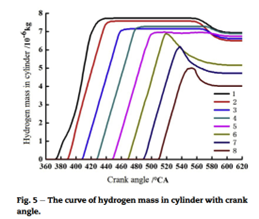
\includegraphics{figures/LR_IT_1.png}}
\caption{Hydrogen Mass}
\label{lr_it_1}
\end{figure}

Similar slopes in the first half – hydrogen enters the cylinder at same rate
Early injection – less amount of backflow. Higher fraction of mass can flow into the cylinder
As the compression stroke starts after 540 CAD, flow of hydrogen from cylinder to intake, backflow generates due to the inertia of the piston. Consequently, hydrogen mass within the cylinder is reduced.  
During the delayed injected cases backflow is much significant.
Trapped hydrogen mass within the cylinder reduces drastically, decreasing the equivalence ratio.

[2] showed that trapped hydrogen mass increases first and then decrease with delayed injection timing. There is an optimum injection timing to trap maximum amount of hydrogen from injected mass.

\begin{figure}[htbp]
    \centerline{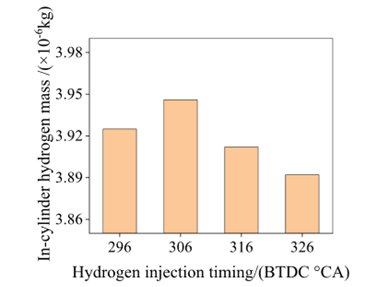
\includegraphics{figures/LR_IT_2.png}}
    \caption{Hydrogen Mass}
    \label{lr_it_2}
    \end{figure}

\begin{figure}[htbp]
        \centerline{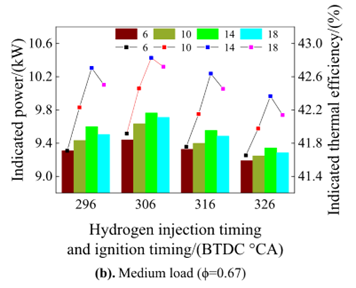
\includegraphics{figures/LR_IT_3.png}}
        \caption{Hydrogen Mass}
        \label{lr_it_3}
        \end{figure}

It can be observed from the graphs that both indicated power and thermal efficiency corelates with trapped hydrogen mass. Both indicated power and indicated thermal efficiency follows a similar trend as trapped hydrogen mass. 
Injection timing affects not only the trapped hydrogen mass but for the local concentration of hydrogen mass near valve seats. Figure [3] shows the relationship between injection timing and local concentration of hydrogen mass near valve seats. A similar study has conducted by [4] and found the similar pattern of increasing local concentration of hydrogen with delaying of injection.
 
\begin{figure}[htbp]
    \centerline{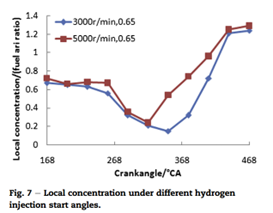
\includegraphics{figures/LR_IT_4.png}}
    \caption{Hydrogen Mass}
    \label{lr_it_4}
    \end{figure}

\begin{figure}[htbp]
    \centerline{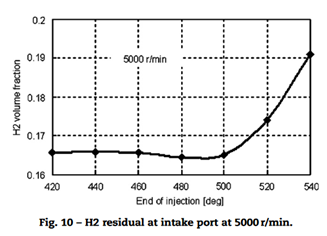
\includegraphics{figures/LR_IT_5.png}}
    \caption{Hydrogen Mass}
    \label{lr_it_5}
    \end{figure}

Too early injection – large amount of hydrogen enters the inlet port and spreads towards the inlet valve before the inlet valve opens. As a result, high concentration of mixture gathers around the intake valve.
Too late injection – hydrogen injection continuous after the intake valve closes, causing high concentration mixture. Hydrogen cannot flow into the cylinder completely.
Proper injection – high concentrated mixture is maintained at a distance from the intake valve. By the time of valve closing, the mixture has already entered the cylinder.

As we can see from the studies, the increment of local concentration is more rapid when delaying injection than with early injection.
In the research conducted by [3], and as shown in the graph, excessively early or delayed injection increases the maximum pressure in the intake port which is an indicate of backfire. In the intermediate injection times, the risk of backfire is minimal. 

\begin{figure}[htbp]
    \centerline{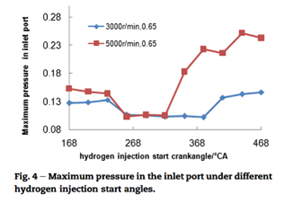
\includegraphics{figures/LR_IT_6.png}}
    \caption{Hydrogen Mass}
    \label{lr_it_6}
    \end{figure}

Comparison of local concentration of hydrogen mass and intake manifold pressure implies that local concentration of hydrogen near valve seats can strongly influence the backfiring risk. 
In brief, literature suggests that trapped hydrogen mass should be maximized to increase performance of the engine while keeping the local concentrations near inlet valve seats at a minimum level to prevent backfire risks.
    
\subsection{Valve Timing}

From the study conducted by [5] we can observe the variation of in-cylinder mass and backflow mass with change of IV timing.

\begin{figure}[htbp]
    \centerline{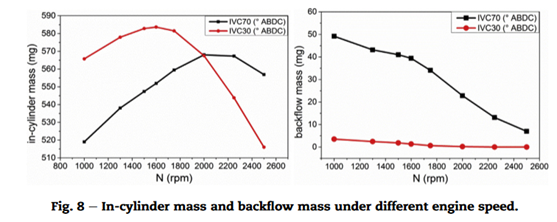
\includegraphics[width=94mm]{figures/LR_VT_1.png}}
    \caption{Hydrogen Mass}
    \label{lr_vt_1}
    \end{figure}

When the engine speed is lower than 2000 rpm, late closing of IV causes a reduction in cylinder mass. This mass reduction is more significant when the engine speed is much lower.
The behavior is opposite with engine speeds higher than 2000 rpm.
Backflow mass is insignificant compared to cylinder mass during the early closure of IV.
However, it is significant when the IVC is retarded. The trend decreases with higher engine speeds.

As mentioned earlier, trapped mass and backflow mass affects engine performance. Increased trapped mass and reduced backflow leads to higher indicated power and efficiency. Therefore, IV timing is an important factor for engine performance.
Study [6] showed the effect of IVO time on engine performance and efficiency for engine speed of 2000 rpm. Torque and efficiency decrease with retarding IVO.

\begin{figure}[htbp]
    \centerline{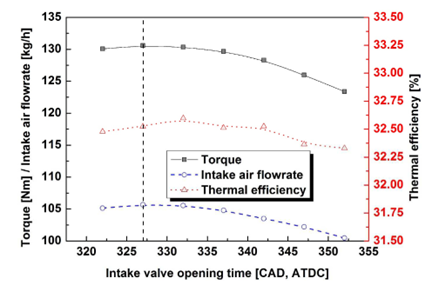
\includegraphics{figures/LR_VT_2.png}}
    \caption{Hydrogen Mass}
    \label{lr_vt_2}
    \end{figure}

[7] studied a wider range of valve overlaps to evaluate engine performance and showed that brake torque reduces in both low and excessive valve overlap times. VOT of 30 seems to be the optimum VOT within the range in terms of engine performance. Further, torque reduction is more significant with reducing valve overlaps than with increasing. 

\begin{figure}[htbp]
    \centerline{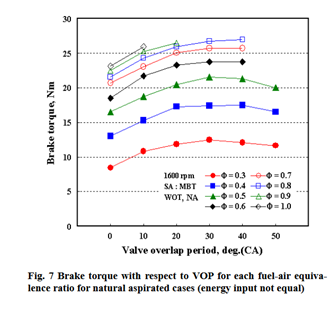
\includegraphics{figures/LR_VT_3.png}}
    \caption{Hydrogen Mass}
    \label{lr_vt_3}
    \end{figure}

In the same study the effect of backfire with valve overlap is studied. Probability of backfire decreased with decrease of valve overlap. That is, valve overlap can be effectively used to control backfire.

\begin{figure}[htbp]
    \centerline{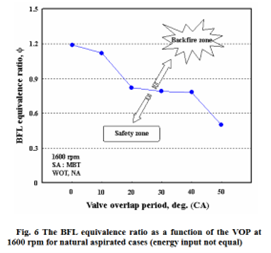
\includegraphics{figures/LR_VT_4.png}}
    \caption{Hydrogen Mass}
    \label{lr_vt_4}
    \end{figure}

This idea of backfire controlling with reducing valve overlap is also mentioned by [8]. The study conducted experiments to show that IVO timing can be used to control backfire with an ultra-lean mixture. Results revealed that with a delay of 100CA, backfire-free operation can be ensured.

\begin{figure}[htbp]
    \centerline{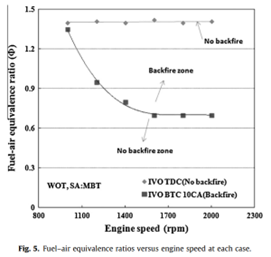
\includegraphics{figures/LR_VT_5.png}}
    \caption{Hydrogen Mass}
    \label{lr_vt_5}
    \end{figure}

\subsection{Combined Effect}

From the evidence above, trapped hydrogen mass and local concentration are highly dependent on both valve and injection timing.  
As [7] stated, combustion characteristics are changed due to mixing and turbulent intensities.
Flow characteristics including turbulent intensities changes the amount of mixing thus the mixture uniformity. Proper mixing reduces the local pockets of high concentrated hydrogen which would otherwise cause abnormal combustion events.
This flow characteristics and mixture uniformity are highly influenced by the combined effect of both valve and injection timing.
Further, since the trapped mass is affected by both valve and injection timing their combined effect is important to trap the correct amount of hydrogen mass within the cylinder, which would give proper combustion characteristics, performance, and efficiency.
The combined effect on combustion characteristics and performance is not well demonstrated yet.


\section*{Acknowledgment}



\begin{thebibliography}{00}
\bibitem{b1} G. Eason, B. Noble, and I. N. Sneddon, ``On certain integrals of Lipschitz-Hankel type involving products of Bessel functions,'' Phil. Trans. Roy. Soc. London, vol. A247, pp. 529--551, April 1955.
\bibitem{b2} J. Clerk Maxwell, A Treatise on Electricity and Magnetism, 3rd ed., vol. 2. Oxford: Clarendon, 1892, pp.68--73.
\bibitem{b3} I. S. Jacobs and C. P. Bean, ``Fine particles, thin films and exchange anisotropy,'' in Magnetism, vol. III, G. T. Rado and H. Suhl, Eds. New York: Academic, 1963, pp. 271--350.
\bibitem{b4} K. Elissa, ``Title of paper if known,'' unpublished.
\bibitem{b5} R. Nicole, ``Title of paper with only first word capitalized,'' J. Name Stand. Abbrev., in press.
\bibitem{b6} Y. Yorozu, M. Hirano, K. Oka, and Y. Tagawa, ``Electron spectroscopy studies on magneto-optical media and plastic substrate interface,'' IEEE Transl. J. Magn. Japan, vol. 2, pp. 740--741, August 1987 [Digests 9th Annual Conf. Magnetics Japan, p. 301, 1982].
\bibitem{b7} M. Young, The Technical Writer's Handbook. Mill Valley, CA: University Science, 1989.
\end{thebibliography}

\end{document}
